\section{Does the Qualified Design Pay? (RQ3)}
\label{sec:cost}
\subsection{RTX: deployment gain and speculative increment}
The RTX expansion measures four conditions in four balanced rounds. Ordinary $R$ uses mask 0/UB1 without draft; matched $M$ uses mask 3/UB4 without draft; candidate $C$ uses mask 3/UB4/$k=3$; the all-scope condition uses mask 15. Each round has four separate resident processes, each with one excluded warmup and 24 formal requests. Condition and task orders rotate; recorded cache reuse is zero. Thus the paths share a panel and campaign but not one simultaneous resident process.

Table~\ref{tab:rtx_cost} reports the same-record CPU reconstruction against both paid baselines. Generation speed is $1.170124\times$ ordinary and $1.169238\times$ matched execution, with 22/24 tasks faster in each comparison. Resident-request speed is $1.741569\times$ ordinary but $1.035071\times$ matched. Crucially, $R/M$ request speed is $1.682560\times$: most of the ordinary-reference request improvement is available without speculation. The $1.742\times$ result is the benefit of the full deployment change and cannot be assigned entirely to speculative execution.

% Generated by scripts/reconstruct.py from frozen exports.
\begin{table}[ht]\centering\small
\caption{RTX frozen expansion paid ratios: 24 task medians, four repeats. Intervals describe task resampling. $C_3$ is mask 3 speculation.}\label{tab:rtx_cost}
\begin{tabular}{@{}lrrrr@{}}\toprule
Ratio & Gen. & Interval & Request & Interval\\\midrule
$R$/$C_3$ & 1.170124 & [1.117,1.218] & 1.741569 & [1.655,1.827]\\
$M$/$C_3$ & 1.169238 & [1.117,1.217] & 1.035071 & [1.005,1.063]\\
$R$/$M$ & 1.000758 & [0.995,1.008] & 1.682560 & [1.590,1.766]\\
\bottomrule\end{tabular}

\end{table}


Figure~\ref{fig:cost} displays the three comparisons on a common baseline/candidate axis while keeping generation and resident-request intervals distinct. Equation~\ref{eq:identity} is verified for all 48 task-level timer identities and both aggregate identities. This consistency check explains why the three ratios fit together; it does not measure which component contributes a fraction of the saving.

\begin{figure}[!htbp]
\centering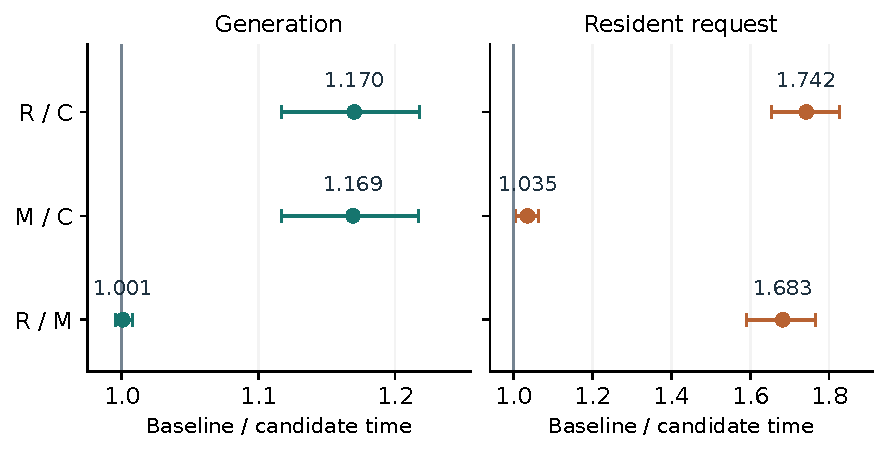
\includegraphics[width=\linewidth]{figures/figure_4_paid_cost.pdf}
\caption{RTX expansion paid speed ratios with descriptive task-bootstrap intervals. Ordinary/candidate measures the deployment change; matched/candidate the increment from speculation; ordinary/matched the draft-free path change. The two timers cover different intervals. Ratios are not additive component costs.}
\label{fig:cost}
\end{figure}

The target-path comparison changes prefill microbatch/attention behavior and continuation capacity jointly. Generation $R/M$ is near parity, whereas the request ratio is much larger. Without independent profiling, that contrast cannot quantify attention, KV, transport, synchronization or host shares. It also cannot certify that $R$ is the fastest ordinary decoder. A faster qualified ordinary implementation could narrow the deployment benefit without changing the arithmetic reported here.

\subsection{Task variation and session uncertainty}
The incremental request benefit is modest and uneven. Figure~\ref{fig:tasks} keeps task generation and request ratios in the same request-sorted order. Seven tasks are slower than matched execution, although all 24 are faster than ordinary request cost. Matched-request round 2 reverses direction at $0.940220\times$; the other round geometric means are approximately 1.029, 1.052 and 1.044. The descriptive task interval for the median-based aggregate lies above one, but does not erase that reversal.

\begin{figure}[!htbp]
\centering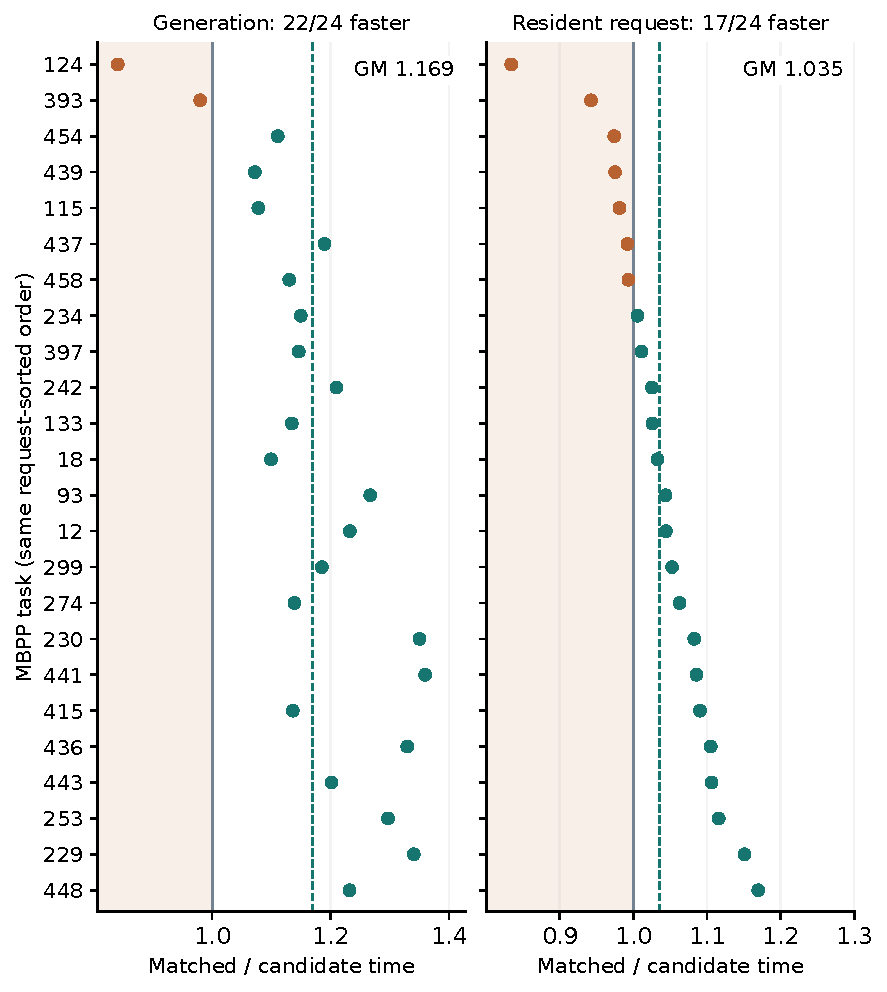
\includegraphics[width=\linewidth]{figures/figure_5_task_variation.pdf}
\caption{RTX matched/candidate task ratios from four-repetition absolute-time medians, in a shared order sorted by request ratio. Points represent tasks. Generation improves on 22/24 and resident request on 17/24; seven request regressions remain. Dashed lines mark aggregate geometric means and the solid parity line marks one.}
\label{fig:tasks}
\end{figure}

Separate resident sessions, laptop scheduling and thermal variation can affect these estimates. Balanced order and task medians reveal some variation but do not remove session confounding. A task bootstrap is not independent session/day replication. We therefore report a qualified positive aggregate operating point, rather than stable production request acceleration. The larger generation gain remains a result for its defined interval, not an end-to-end substitute.

The serial resident-reset study supplies a separate finite check: recorded requests begin with reset target state and the original $k=3$/UB4 recipe retains reference output across two request orders. Its matched generation/request speeds are about $1.181\times/1.039\times$. This supports the registered reset behavior. It is not a concurrency or throughput experiment and is not pooled with the 384 expansion rows.

\subsection{Fixed UB: wider drafting qualifies but becomes slower}
The geometry failures in Section~\ref{sec:repair} change $k$ and UB together. A separate frozen experiment holds UB4 and mask 3 fixed while testing $k=3,5,7$ on 24 now-exposed MBPP inputs plus four exposed HumanEval probes. All widths qualify in two repetitions. The highest passing $k=7$ is selected by qualification alone, then measured in separate capture-off sessions: four conditions, four repetitions and 448 formal requests. Qualification timings are excluded from speed selection.

Relative to the $k=3$ anchor, $k=7$ reaches only $0.829442\times$ generation and $0.889868\times$ resident-request speed. Against matched target-only, it reaches $0.997404\times/0.950353\times$, while the anchor reaches $1.202501\times/1.067970\times$ in that campaign. The widened candidate preserves the reference and fails the extra-cost objective. Ordinary same-width speculation has output failures, so its times remain diagnostic rather than qualified speed evidence.

Formal draft work grows from 3,528 to 5,392 tokens while accepted draft tokens grow from 2,772 to 3,192. In separate captured qualification sessions, target continuation caller calls fall from 305 to 199, but observed micrographs rise from 305 to 397. These sessions include their own warmups and forced synchronization; the counts cannot be combined with formal times into a fabricated per-call profile. Micrographs are not CUDA kernel launches. The evidence rejects caller reduction as a sufficient performance proxy without assigning the slowdown to a unique component.

Saved partitions also matter. At $k=7$, matched generation/request speed is $0.953/0.919\times$ on 24 MBPP inputs but $1.308/1.164\times$ on four HumanEval probes. The pooled result hides these differences. Four exposed probes do not validate a routing rule, and no online selector was developed from them. S1 retains the longer-cap confirmation and the failed wider-geometry branches without combining their timers into an optimization trajectory.

\subsection{B570: repair improves an old path but loses to strong baselines}
The B570 formal matrix remains 119/120 complete: old N1's first-round MBPP/400 payload is missing after an infrastructure interruption. No request is imputed or rerun in the scientific denominator. Ordinary $R$, matched $M$ and candidate $C$ each have 30 complete responses, providing 15 two-round task-median pairs. Old-N1 comparisons have 14 complete task pairs.

Table~\ref{tab:b570_cost} gives all three timers. Candidate speed is $0.282588\times$ generation and $0.201290\times$ whole request against ordinary $R$, and $0.285761\times/0.205704\times$ against matched target-only. Both baselines are faster in every available paired round. The matched target path is close to ordinary cost ($R/M=0.988893\times/0.978539\times$), so the roughly fivefold candidate request cost cannot be attributed entirely to the consistency constraint on the target path.

% Generated by scripts/reconstruct.py from frozen exports.
\begin{table}[ht]\centering\small
\caption{B570 paid baseline/candidate task-median ratios. Complete two-round pairs only; the missing old-N1 task is not imputed. All raw suffix work stays charged.}\label{tab:b570_cost}
\begin{tabular}{@{}lrrrr@{}}\toprule
Ratio & Tasks & Generation & Whole request & Host\\\midrule
$R/C$ & 15 & 0.282588 & 0.201290 & 0.201884\\
$M/C$ & 15 & 0.285761 & 0.205704 & 0.206243\\
Old N1/$C$ & 14 & 3.993091 & 2.633940 & 2.633387\\
$R/M$ & 15 & 0.988893 & 0.978539 & 0.978864\\
\bottomrule\end{tabular}

\end{table}


Against old N1, the candidate improves generation/request speed by $3.993091\times/2.633940\times$ over 14 task pairs. That is real engineering progress relative to a slow prior frontend, but does not establish deployment benefit. MBPP/245 also reverses the old-path request comparison in round 2. Neither aggregate improvement nor endpoint recovery supports a universal per-round gain.

The candidate's formal records contain 888 drafted and 702 accepted tokens. Endpoint IDs total 1,150 while raw IDs total 1,176; all 26 suffix IDs remain charged. Target and draft continuation caller-token totals are 1,332 and 1,362. These are distinct runtime quantities. Raw suffix equality is not required by this endpoint contract and is not claimed. Removing witness readbacks, an extra context and handoff improves the frontend, while phase reservation, synchronization, drafting and rollback remain online. No full independent component profile identifies a unique remaining bottleneck. The appropriate decision is to reject this recipe as a latency improvement against the two strong baselines.

\subsection{Global serialization, control, and draft-side limits}
An earlier RTX global-serialization timing arm qualifies 57/57 arrays on 19 exposed tasks but reaches only $0.677351\times$ target-only speed, with descriptive interval approximately $[0.662,0.692]$ and zero tasks faster. Its synchronized post-prefill-to-slot-release interval includes instrumented work and logging, unlike the later server generation field. It is a separate qualified cost failure, not the first point of a common before/after speed curve. S1 preserves its host-timer amendment and the preceding V3 stop.

M4 provides a contrasting control decision under its own contract. A prospective 60-task, three-condition, three-repeat campaign has 540 requests; both fixed Always speculation and Guard qualify 180/180 direct generated-ID comparisons. Against target-only, their post-prefill speeds are $1.346894\times$ and $1.311387\times$. A paired secondary analysis gives Guard/Always latency $1.027076$, with descriptive interval $[1.012956,1.043559]$: this guard is slower on the measured comparison. It should not be retained on the premise that adaptivity necessarily improves performance.

A hindsight per-task oracle choosing only target-only or Always leaves about 0.069\% further geometric-mean latency reduction relative to Always. This is a panel-specific two-action opportunity, not an upper bound on intra-request policies. HumanEval and Spec-Bench fixed-policy speeds also differ ($1.570\times$ versus $1.155\times$). The formal direct-ID study is distinct from earlier M4 text-based and proxy measurements.

On 358H, CPU/NPU drafting each qualifies its 90-request direct-ID panel but yields $0.733915\times/0.351663\times$ speed. With baseline cost $B_{ij}$, measured target work $T_{ij}$ and progress fixed, removing all other nonnegative work gives the conditional budget
\begin{equation}
\operatorname{GM}_{i}\operatorname{median}_{j} S'_{ij}
\leq \operatorname{GM}_{i}\operatorname{median}_{j}(B_{ij}/T_{ij}).
\label{eq:floor}
\end{equation}
Prompt-estimator ceilings are $0.8372\times/0.8448\times$, still below parity. Even deleting all other work would require a uniform target-work reduction of at least 16.28\%/15.52\% to reach parity under that estimator. Pooled-total ceilings differ and remain in S1. Full-prefix NPU replay is an implementation cost, not a theorem against heterogeneous inference. This case redirects optimization toward target work or a different state interface; faster isolated drafting alone cannot meet the measured budget.
